
%%%%%%%%%%%%%%%%%%%%%
\chapter{Ensemble et application}
%%%%%%%%%%%%%%%%%%%%%

%%%%%%%%%%%%%%%%%%%%%%%%%
\section{Ensemble}
%%%%%%%%%%%%%%%%%%%%%%%%%
%$\mathcal{}$
Un ensemble est une collection d'objets. Un objet (a) appartenant à un ensemble ($\mathcal{A}$) est appelé élément de l'ensemble.

L'élément a appartient à l'ensemble ($\mathcal{A}$) s'écrit :

\[
 a \in \mathcal{A}
\]

Un ensemble peut être représenté par une enveloppe autour de ses éléments représentés par des points :



\begin{center}
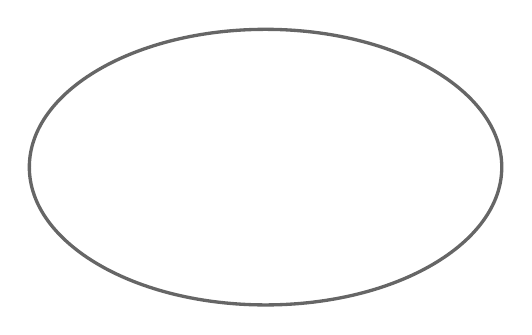
\begin{tikzpicture}

	\def\a{3} \def\b{1.75} % Taille de l'ellipse
\draw[black!60,very thick]
		(0,0) circle[x radius = \a cm, y radius = \b cm];

	\def\i{0.85} \def\j{-0.25}% Position relative des points
	
\end{tikzpicture}
\end{center}

    \begin{tikzpicture}[scale=1.2]
	\tikzset{mypoints/.style={fill=white,draw=black,thick}}
	\def\ptsize{2.0pt}
	\def\a{3} \def\b{1.75}
	% warning: construction fails if xp<0 or yp<=0
	\def\xp{4.0} \def\yp{3.5} 
	\def\i{0.85} \def\j{-0.25}%determines rays from P
	\coordinate[label=above:P] (P) at (\xp,\yp);
	\coordinate (M) at ({\a*\i},0);
	\coordinate (N) at ({\a*\j},0);
	\coordinate (AA) at (0,-\b);
	\coordinate (BB) at (1,-\b);
	\coordinate (CC) at (-\a,0);
	\coordinate (DD) at (-\a,1);
	\coordinate (Q) at (intersection of P--N and AA--BB);
	\coordinate (R) at (intersection of P--M and AA--BB);
	%\draw[name path=ellipse,red,very thick]
		(0,0) circle[x radius = \a cm, y radius = \b cm];
	%\path[name path=linePQ,blue] (P)--(Q);
	%\path[name path=linePR,green] (P)--(R);
	%\path [name intersections={of = ellipse and linePQ}];
	%\coordinate[label=above:A] (A)  at (intersection-1);
	%\coordinate[label=below left:B] (B) at (intersection-2);
	%\path [name intersections={of = ellipse and linePR}];
	%\coordinate[label=above right:C] (C)  at (intersection-1);
	%\coordinate[label=above left:D] (D) at (intersection-2);
	%\draw (B)--(P)--(D) (A)--(D) (C)--(B);
	%\coordinate [label=below left:E] (E) at (intersection of A--D and B--C);
	%\coordinate[label=above right:F] (F) at (intersection of A--C and B--D);
	%\coordinate (G) at (intersection of E--F and CC--DD);
	%\draw [name path=lineFG,blue,thick] (F)--(G);
	%\draw (A)--(F)--(B);
	%\path [name intersections={of = ellipse and lineFG}];
	%\coordinate[label=above:X] (X) at (intersection-1);
	%\coordinate[label=above right:Y] (Y) at (intersection-2);
	%\coordinate (XX) at ($(P)!1.5!(X)$);
	%\coordinate (YY) at ($(P)!1.5!(Y)$);
	%\draw[very thick,green!50!black!50] (XX)--(P)--(YY);
	%\foreach \p in {A,B,C,D,E,F,P,X,Y}\fill[mypoints] (\p) circle (\ptsize);
  \end{tikzpicture}
%%%%%%%%%%%%%%%%%%%%%%%%%
\section{Application}
%%%%%%%%%%%%%%%%%%%%%%%%%
Une application ($f$) met en relation des éléments ($a$) d'un ensemble ($\mathcal{A}$, dit de départ) avec des éléments ($b$) d'un autre ensemble ($\mathcal{B}$, dit d'arrivé). :
\begin{align*}
f :\ \ \ \ \ \ \ \ \ \mathcal{A} \ \  & \rightarrow \ \ \ \mathcal{B} \\
a \ \ & \mapsto \ \ b = f(a)
\end{align*}

Une loi de composition est une application qui associe deux éléments (éventuellement du même ensemble) à un troisième élément. 
\begin{align*}
f :\ \ \ \ \ \ \ \ \ \mathcal{A} \times \mathcal{B} \ \  & \rightarrow \ \ \ \mathcal{C} \\
(a,b) \ \ & \mapsto \ \ c = f(a,b)
\end{align*}

Une loi de composition est dite interne si $\mathcal{A} = \mathcal{B} = \mathcal{C}$, externe sinon.

%%%%%%%%%%%%%%%%%%%%%%%%%%%%%%%%%%%%%%%%%%%%%%%%%%%%%%%%%%%%%%%%%%%%%%%%%%%%%%%%%%%%%
